% !TeX spellcheck = en_US
% !TeX root = ../BachelorThesis.tex

\section{Resting Heart Rate}
Every minute, the heart rate of a participant is measured by the activity tracker and eventually stored in the database. 
In \Cref{table: Heartrate Analysis}, we see the heart rates of our participants.
The corresponding plots can be seen in \Cref{fig: heart rates plots}.
As one can notice, not all the dates visible in each of the boxplots in \Cref{fig: heart rates boxplots} are in these plots. 
This is because all participants did not give a rating for some days.
Although we do not know for sure why this is the case, this is probably because they forgot to do so.
We also excluded these days without ratings in each of the tables in \Cref{table: Heartrate Analysis}.
In contrary to our first investigated biomarker (2MWT), we can see that a lot more measurements are present in \Cref{fig: heart rates plots}.
Because each device automatically measures the heart rate, there is no user intervention required which definitely has a positive effect on the amount of data.

If we take a look at the boxplots in \Cref{fig: heart rates boxplots}, we see that the majority of the fliers (outliers) are in the high regions of the boxplots.
In the lower parts, we rarely see fliers.
This observation gave us the insight that the average of the lowest 5\% of the measurements is probably a good and stable estimation of the resting heart rate of the participant for a single day.
Therefore, the plots show the average of the lowest 5\% of the heart rates measurements and not the average of all the measurements for that day.
For each participant, Kendall's $\tau$ correlation coefficient along with the $p$-values can be seen in \Cref{table:resting heart rate kendall tau}.
As we have seen in \Cref{section:Resting Heart Rate}, the resting heart rate for adult lies between 60 and 100 beats, which is also suggested by the figures in \Cref{fig: heart rates plots}.
In \Cref{section:Resting Heart Rate}, we have also seen that a low resting heart rate is more desirable than a high one.
Looking at the plot from participant \subref{fig:heart user2}, we see exactly the opposite of what we would have expected: for most of the lower resting heart rates, the day ratings tend to go worse. 
The day on which the participant had his lowest resting heart rate was rated as `bad'.
For participant \subref{fig:heart user1}, such a relation is not visible as the data seems to be spread randomly.

In \Cref{table:resting heart rate kendall tau}, we see that the correlation coefficient for participant \subref{fig:heart user3} is close to zero.
The coefficients for participants \subref{fig:heart user2} and \subref{fig:heart user4} tend to go negative, suggesting that if the rank of the average of the lowest 5\% of the heart rate measurements decreases, the rank of the rating increases (which we also noticed by ourselves). 
None of the $p$-values is near 0.05.
This indicates that the effect observed in the data is likely, even assuming that the null hypothesis of no effect is true.
For this particular biomarker, the null hypothesis would state that there is no relation between the average of the lowest 5\% of the heart rates and the rating of the day after.
%
\newpage
\begin{table}[H]
	\centering
	\begin{tabular}{@{}lll@{}}
		\toprule
		\textbf{Participant} & \bm{$\tau$} & \bm{$p$}\\
		\midrule
		\subref{fig:heart user1} & $0.128873$ & $0.254708$ \\
		\subref{fig:heart user2} & $-0.176887$ & $0.305310$ \\
		\subref{fig:heart user3} & $0.021340$ & $0.842163$ \\
		\subref{fig:heart user4} & $-0.174944$ & $0.210129$ \\
		\bottomrule
	\end{tabular}
	
	\captionof{table}{Expressing the rank correlation between the average of the lowest 5\% of the heart rate measurements and the day rating.
	}
	\label{table:resting heart rate kendall tau}
\end{table}
%
\begin{figure}[H]
	\centering
	\subfloat[]{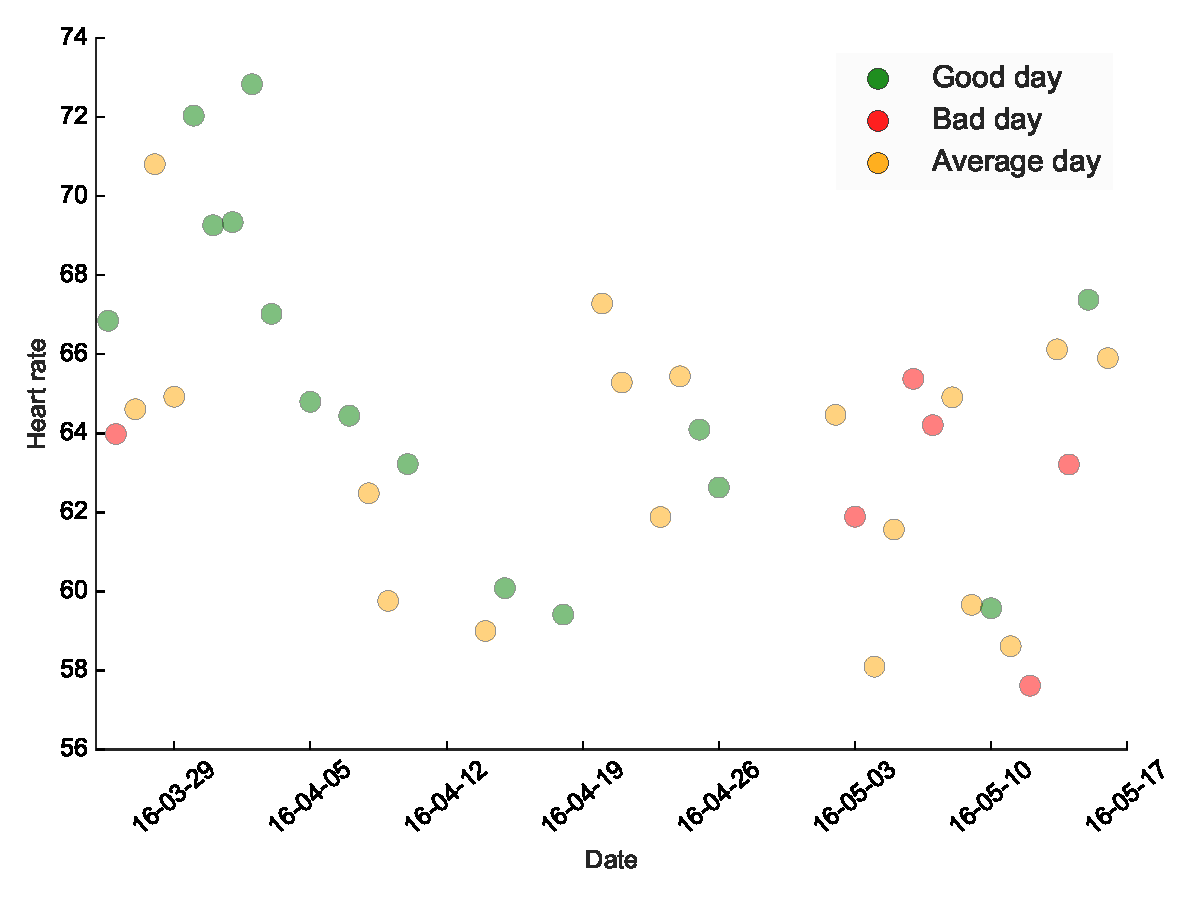
\includegraphics[scale=0.29]{img/heartrate/2Dy2uFf3aw6jv9r5u}
		\label{fig:heart user1}
	}
	\hspace{0.5cm}
	\subfloat[]{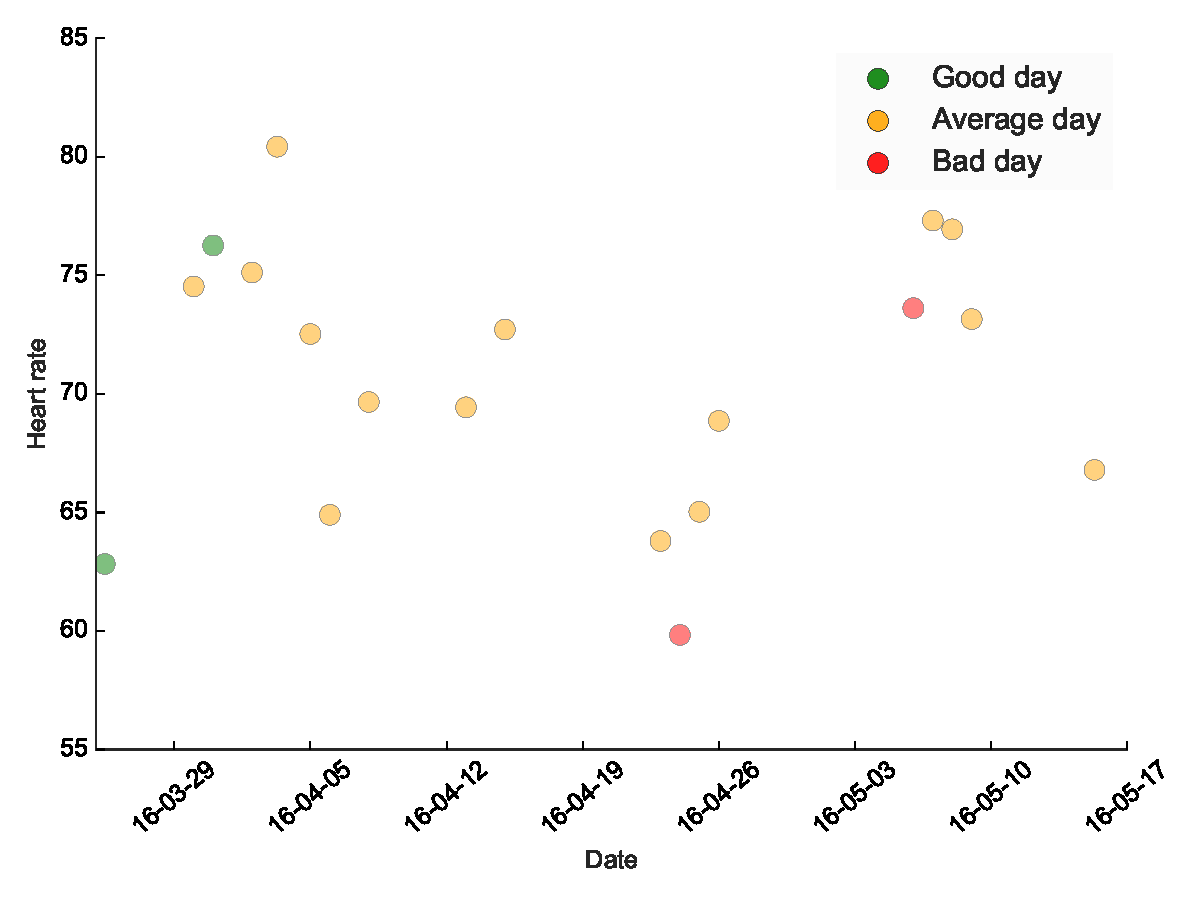
\includegraphics[scale=0.29]{img/heartrate/dW4YzJQEaidmyhsuY}
		\label{fig:heart user2}
	}
	\vfill
	\subfloat[]{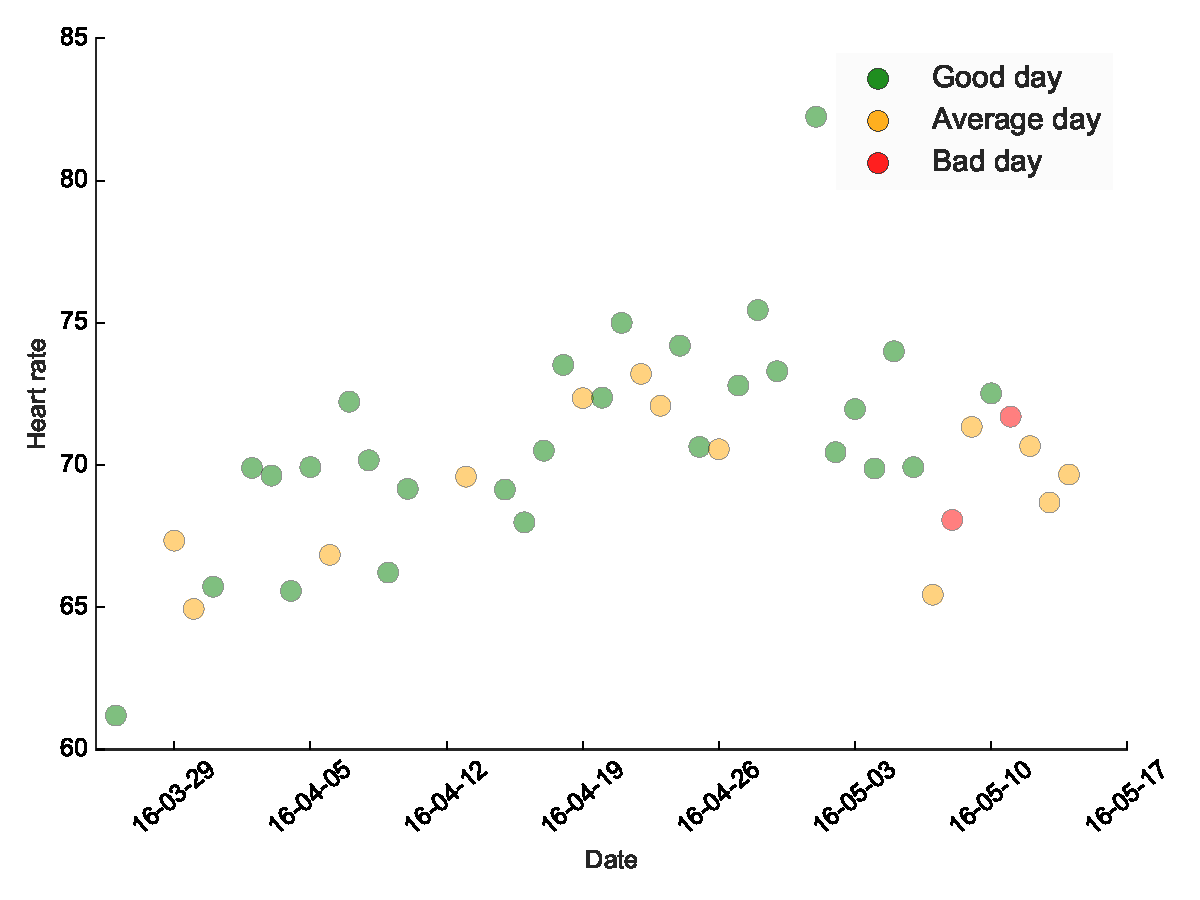
\includegraphics[scale=0.29]{img/heartrate/gGSWzh5PnqgFdCpq4}
		\label{fig:heart user3}
	}
	\hspace{0.5cm}
	\subfloat[]{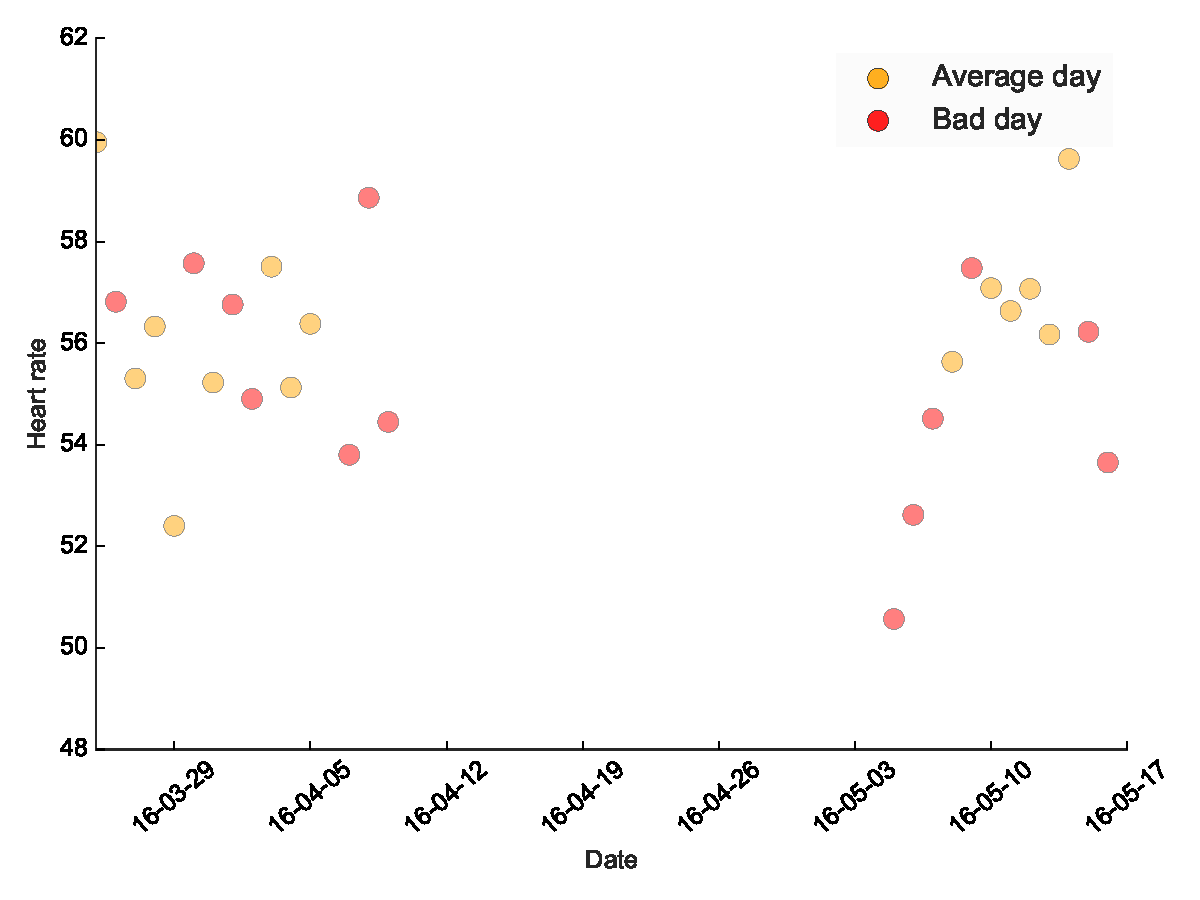
\includegraphics[scale=0.29]{img/heartrate/S2usWtx8WXPe8S88r}
		\label{fig:heart user4}
	}
	\captionof{figure}{Plots of the average from the lowest 5\% of the heart rates measurement of the participants for each day. 
	Only dates that both had a rating and measurements of heart rates are shown. 
	As can be seen in the legend of each of the figures, each point is colored according to the rating given by the participant for that day.}
	\label{fig: heart rates plots}
\end{figure}
\newpage
%